\documentclass{article}
\usepackage{qilin}
\tikzstyle{process} = [rectangle, rounded corners, minimum width=1.5cm, minimum height=0.5cm,align=center, draw=black, fill=gray!30, auto]
\title{CHE260: Heat Transfer}
\author{QiLin Xue and John Zhang}
\date{Fall 2021}
\usepackage{mathrsfs}
\usetikzlibrary{arrows}
\begin{document}

\maketitle
% \section{Mechanisms of Heat Transfer}
% \begin{itemize}
%         \item Mechanisms involve:
%         \begin{itemize}
%             \item Conduction: Transfer of heat through a medium that is stationary.
%             \item Convection: Transfer of heat from a solid surface and an adjacent fluid that is moving.
%             \item Radiation: Energy emitted by matter in the form of electromagnetic waves.
%         \end{itemize}
%         \item Conduction follows \textbf{Fourier's Law:}
%         \begin{equation}
%             \dot{Q} = - k A \nabla T
%         \end{equation}
%         \item The rate of heat transfer from the surface of a blackbody is given by the Stefan-Boltzmann Law 
%         \begin{equation}
%             \dot{Q}_\text{emit,max} = \sigma A T_s^4
%         \end{equation}
%         where $\sigma$ is the Boltzmann constant $\sigma = 5.67 \times 10^{-8} \frac{W}{m^2 K^4}$
%         \item For an ideal body, we have
%         \begin{equation}
%             \dot{Q}_\text{emit} = \epsilon \sigma AT_s^4
%         \end{equation}
%         where $0 \le \epsilon \le 1$ is the emissivity.
%         \item When radiation is incident on a surface, some will be absorbed and some reflected. The \textbf{absorptivity} $\alpha$ is defined such that
%         \begin{align}
%             \dot{Q}_\text{absorbed} &= \alpha \dot{Q}_\text{incident} \\ 
%             \dot{Q}_\text{reflected} &= (1-\alpha)\dot{Q}_\text{incident}
%         \end{align}
%         \item Kirchoff's Law says that
%         \begin{equation}
%             \alpha = \epsilon
%         \end{equation}
%         \item For a small surface completed surrounded by a much larger surface net radiation is 
%         \begin{equation}
%             \dot{Q}_\text{net} = \epsilon \sigma A (T_s^4 - T_\text{surrounding}^4)
%         \end{equation}
%         \item Natural convection tells us the heat transfer coefficient is
%         \begin{equation}
%             h = c(T_S-T_\infty)^{1/4}
%         \end{equation}
%         where $c=4.2 \text{W}{m^2 K^{5/4}}$ and 
%         \begin{equation}
%             q_\text{conv}  = hA(T_S-T_\infty)
%         \end{equation}
%         \item Forced convection gives a constant $h = 250 W/m^2 K$
%         \item Let's look at the \textbf{one-dimensional case:} If we look at a segment of length $\Delta x$, the rate of the increase of enthalpy is
%         \begin{align}
%             \dot{H} &= mc_p \frac{\partial T}{\partial t} \\ 
%             &= \rho c_p A \Delta x \frac{\partial T}{\partial t}
%         \end{align}
%         The energy balance in this small segment gives
%         \begin{align}
%             \rho c_p A\Delta x\frac{\partial T}{\partial t} &= \dot{Q}_x - \dot{Q}_{x+\Delta x} \\ 
%             &= (\dot{q}A)_x - (\dot{q}A)_{x+\Delta x}
%         \end{align}
%         Dividing by $\Delta x$ and taking the limit gives 
%         \begin{equation}
%             \rho c_p \frac{\partial T}{\partial t} = -\frac{1}{A} \frac{\partial(\dot{q}A)}{\partial x}
%         \end{equation}
%         Note that $A$ depends on the coordinate system, $\dot{q}$ depends on Fourier's Law $\dot{q} = -k\frac{dT}{dx}$.
%         \item This gives us the heat conduction equation 
%         \begin{equation}
%             \frac{\partial^2 T}{\partial x^2} = \frac{1}{\alpha}\frac{\partial T}{\partial t}  
%         \end{equation}
%         where $\alpha=\frac{k}{\rho c_p}$ is the thermal diffusivity.
%         \item At constant state, $\frac{\partial T}{\partial t} = 0$, so 
%         \begin{equation}
%             \frac{d^2 T}{dx^2} = 0
%         \end{equation}
%         \item In cylindrical coordinates, we have
%         \begin{equation}
%             \frac{1}{\alpha}\frac{\partial T}{\partial t} = \frac{1}{r}\frac{\partial}{\partial r}\left(r\frac{\partial T}{\partial r}\right)
%         \end{equation}
%         \item In spherical coordinates 
%         \begin{equation}
%             \frac{1}{\alpha}\frac{\partial T}{\partial t} = \frac{1}{r^2}\frac{\partial}{\partial r}\left(r^2 \frac{\partial T}{\partial r}\right)
%         \end{equation}
%         \item In general, we have 
%         \begin{equation}
%             \frac{1}{r^n}\frac{\partial}{\partial r}\left(r^n \frac{\partial T}{\partial r}\right) = \frac{1}{\alpha}\frac{\partial T}{\partial t}
%         \end{equation}
%         where 
%         \begin{itemize}
%             \item $n=0$ for cartesian
%             \item $n=1$ for cylindrical 
%             \item $n=2$ for spherical
%         \end{itemize}
%         \begin{idea}
%             These equations can alternatively derived by applying the divergence formula in different coordinate systems. In particular, it is done by considering the heat equation 
%             \begin{equation}
%                 \frac{1}{\alpha}\frac{\partial T}{\partial t} = \nabla \cdot T
%             \end{equation}
%             and applying spherical / cylindrical symmetry.
%         \end{idea}
%         \item To solve problems, we also need boundary conditions, and we often make the steady state assumption.
%     \end{itemize}


% \section{Thermal resistance Networks and Contact resistance}
% read Chapter 17.2, 17.3

% We can think of a wall with a temperature difference across the two sides as a \textbf{thermal resistor} with a thermal resistance of $r_1 = \frac{T_1 - T_2}{\dot{Q}}$.

% In this way, we can put thermal resistors in series and get the equivalent thermal resistance as:

% $r_{equivalent} = \sum_{i} {r_i}$

% What about the situation where there are three materials stacked up on top of each other bridging two different temperatures, each with their own cross-sectional area?

% If we call the amount of heat transfer in each of these $\dot{Q}_1$, $\dot{Q}_2$, $\dot{Q}_3$, then the total heat transfer is

% $\dot{Q} = \dot{Q}_1 + \dot{Q}_2 + \dot{Q}_3$

% $\dot{Q} = \frac{T_1 - T_2}{\dot{r}_1} + \frac{T_1 - T_2}{\dot{r}_2} + \frac{T_1 - T_2}{\dot{r}_3}$

% = $(T_1 - T_2)[\frac{1}{r_1} + \frac{1}{r_2} + \frac{1}{r_3}]$

% = $\frac{T_1 - T_2}{r_{total}}$

% So our electrical analogy fits thermal resistance completely. Now we can apply this analogy on networks of thermal resistance.

% % \makebox[\textwidth]{\includegraphics[width=\paperwidth]{images/Thermal - electrical network.png}}

% However, a surface in real life is never completely smooth so never has a perfect contact. Between two rough surfaces, air is trapped and affects the heat conduction.

% Heat flux $\dot{q}$ $[\frac{w}{m^2}]$

% Define a thermal contact resistance
% $r_c = \frac{\delta T}{\dot{q}}$ $[\frac{m^2 * C}{W}]$

% Which is the resistance per unit area.

% reciprocal of $r_c$ is the $h_c$, the "thermal contact conductance".

% $h = \frac{1}{r_c} = \frac{\dot{q}}{\delta T}$

% $\dot{q} = h_c \delta T$

% Typical values of $h_c$:

% \begin{center}
% \begin{tabular}{||c c||} 
%  \hline
%  Metal Pairs & $h_c$ ($\frac{w}{m^2 * C}$) \\ [0.5ex] 
%  \hline\hline
%  Steel/Steel & ~$10^3$ \\ 
%  \hline
%  Al/Al & ~$10^4$ \\
%  \hline
%  Cu/Cu & ~$10^5$ \\
%  \hline
% \end{tabular}
% \end{center}

% \section{Contact resistance in Cylinders and Spheres}


% % \makebox[\textwidth]{\includegraphics[width=\paperwidth]{images/Cylinder.png}}

% For a long pipe, $\frac{dT}{dZ} << \frac{dT}{dr}$.
% So we approximate by assuming 1-dimensional conduction in the Z direction.

% $\frac{\partial}{\partial r}(r\frac{\partial T}{\partial r}) = 0$

% Boundary conditions:\\
% $r = r_1, T = T_1$ \\
% $r = r_2, T = T_2$
% \\
% \\

% Integrate:

% $r \frac{dT}{dr} = c_1$\\

% $\rightarrow \frac{dT}{dr} = \frac{c_1}{r}$\\
% $T(r) = c_1 ln(r) + c_2$\\
% \\

% Applying boundary conditions:

% $ T_1 = c_1 ln(r_1) + c_2$\\
% $ T_2 = c_1 ln(r_2) + c_2$\\
% \\

% $\rightarrow T_1 - T_2 = c_1[ln(r_1) - ln(r_2)]$ \\
% $\rightarrow c_1 = \frac{T_1 - T_2}{ln(\frac{r_1}{r_2})}$ \\
% $T_2 = \frac{T_1 - T_2}{ln(\frac{r_1}{r_2})}ln(r_2) + c_2$ \\
% $c_2 = T_2 - \frac{(T_1 - T_2}{ln(\frac{r_1}{r_2})} ln(r_2)$ \\


% $T(r) = \frac{T_1 - T_2}{ln(\frac{r_1}{r_2})} ln(r) - \frac{T_1 - T_2}{ln(\frac{r_1}{r_2})} ln(r_2) + T_2$ \\

% $T(r) = \frac{T_1 - T_2}{ln(\frac{r_1}{r_2})} ln(\frac{r}{r_2}) + T_2$ \\

% $\dot{Q}_{conduction} = -kA_1 \frac{dT}{dr}|_{(r = r_2)}$ \\
% $A_1 = 2\pi r_1 L$

% $\frac{dT}{dr}|_{(r = r_2)} = \frac{T_1 - T_2}{ln(\frac{r_1}{r_2})} ln(\frac{r_2}{r} - \frac{1}{r_2})|_{r = r_1}$

% Finally:
% $\dot{Q}_{conduction} = 2\pi L k \frac{T_1 - T_2}{ln(\frac{r_1}{r_2})})$

% Define thermal resistance of a cylinder:
% $r_{cylinder} = \frac{T_1 - T_2}{\dot{Q}_{conduction}}$
% $r_{cylinder} = \frac{ln(r_2/r_1)}{2\pi Lk}$

% For a sphere:
% $r_{sphere} = \frac{r_2 - r_1}{4\pi r_1 r_2 k}$

% \section{Conduction in Cylinders and Spheres}
% Let $h_1$ be the thermal contact conductance between the outer surface of the cylinder and the outer surface of the sphere. 
\section{Introduction}
\textit{Covers 1.1: Mathematical Models and Solutions}
\begin{itemize}
    \item Big Idea: Differential equations model physical situations:
          \begin{itemize}
              \item Take a physical situation and ODE-ify it (How do we model a cooling coffee cup?)
              \item Understand an ODE without solving it (What can we deduce directly from $y'=y^2$?)
              \item Study, categories, typecast ODEs and solve them
                    \begin{example}
                        Suppose we have $y'=y/t+\ln t$ and $y'=y^2+t$. Which of these are harder to solve (without actually solving them)?
                        \vspace{2mm}

                        It turns out that the second one is harder as it is \textit{non-linear}.
                    \end{example}
              \item Handle ODEs numerically (What do we do when we cannot solve an ODE that models a real life phenomenon?)
              \item The art of problem solving (How do I work with no strings attached?)
          \end{itemize}
    \item What is a differential equation?
          \begin{definition}
              A differential equation relates a function and its derivatives.
          \end{definition}
    \item We can understand ODEs without solving it:
          \begin{example}
              Let's consider a cup of coffee in a room. We want to model its change in temperature over time. How do we do this?
              \vspace{2mm}

              There are a lot of variables, so we have to simplify our model. The things we care about
              \begin{itemize}
                  \item The temperature of the coffee cup $y(t)$.
                  \item $t$ is in minutes.
                  \item $y(t)$ is in Celsius.
                  \item The temperature in the room $T$ (in Celsius).
              \end{itemize}
              The things we ignore / simplify:
              \begin{itemize}
                  \item Temperature variation within the cup
                  \item Temperature variation in the room
              \end{itemize}
              \textbf{Exercise:} Let's consider some suggestions for an ODE describing the temperature of a coffee cup in a room. Each of the following suggested ODEs contradicts our intuition in some way. How?

              \begin{itemize}
                  \item $y'=y^2$
                        \begin{itemize}
                            \item $T$ isn't in there
                            \item Temperature would always increase except if $y=0$.
                            \item The hotter the coffee, the faster it heats up.
                        \end{itemize}
                  \item $y'=\frac{T}{y}$
                        \begin{itemize}
                            \item If $T>0, y>0$, then $y'>0$
                            \item The model doesn't work for coffee at $0^\circ \text{C}$.
                        \end{itemize}
                  \item $y'=y[e^{y-T}+y^3]$
                  \item $y'=y-T$
                  \item $y'=T-y$
                        \begin{itemize}
                            \item There should be a parameter that describes the physical properties (rate of heating/cooling will be different for different materials)
                        \end{itemize}
              \end{itemize}
          \end{example}
          \begin{idea}
              Without solving an ODE, you can already make many predictions about its solution
              \vspace{2mm}

              (and then, for example, judge your model)
          \end{idea}
    \item We introduce a few definitions
          \begin{definition}
              An \textbf{ordinary differential equation} (ODE) only considers a function of $1$ variable and its derivatives
          \end{definition}
          \begin{definition}
              A \textbf{partial differential equation} considers a function of several variables and its derivatives.
          \end{definition}
    \item The most general ODE for a function $y(t)$ is:
          \begin{enumerate}[label=(\alph*)]
              \item $F[t,y,y'',\dots,y^{(n)}]$ for $n\in \mathbb{N}$.
              \item Any function that satisfies this equation is called \textit{a solution}
          \end{enumerate}
          \begin{definition}
              The order of an ODE is the highest derivative of an ODE.
          \end{definition}
    \item An autonomous ODE is if the independent variable doesn't appear in the ODE.
    \item Systems of ODEs arise if we study several quantities depending on the same variable and how their changes interact.
          \begin{example}
              Assume that $p(t)$ and $o(t)$ describe the number of twitter followers of two accounts. If there is no interaction, what are reasonable ODEs for these two quantities?
              \begin{align}
                  p'(t) = kp(t) \\
                  o'(t) = \ell o(t)
              \end{align}
              Suppose that if in addition to ``word of mouth,'' we consider the effects that these two tweets have, what are reasonable ODEs for the number of followers?
              \begin{align}
                  p'(t) = k \cdot p(t) - m \cdot o(t) \\
                  o'(t) = \ell \cdot o(t) - n \cdot p(t)
              \end{align}
              where all constant are positive. However, this is oversimplified as it assumes the people who follow \textit{O} also follow \textit{P.}
          \end{example}
    \item Suppose a differential equation is given by
          \begin{equation}
              y'(t) = -1.5(y(t)-1)
          \end{equation}
          \begin{definition}
              Consider the ODE $y'=f(t,y)$. We can draw a \textbf{direction field} as follows:
              \begin{enumerate}
                  \item Draw a $t-y$ coordinate system.
                  \item Evaluate $f(t,y)$ over a rectangular grid of points.
                  \item Draw a line at each point $(t,y)$ of the grid with slope $f(t,y)$.
              \end{enumerate}
          \end{definition}
          \begin{center}
              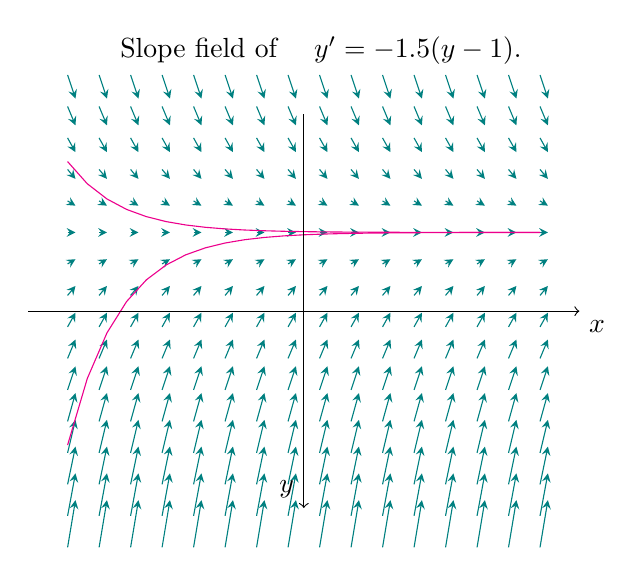
\begin{tikzpicture}[declare function={f(\x,\y)=-1.5*(\y-1);}]
                  \def\xmax{3} \def\xmin{-3}
                  \def\ymax{-3} \def\ymin{3}
                  \def\nx{15}  \def\ny{15}

                  \pgfmathsetmacro{\hx}{(\xmax-\xmin)/\nx}
                  \pgfmathsetmacro{\hy}{(\ymax-\ymin)/\ny}
                  \foreach \i in {0,...,\nx}
                  \foreach \j in {0,...,\ny}{
                          \pgfmathsetmacro{\yprime}{f({\xmin+\i*\hx},{\ymin+\j*\hy})}
                          \draw[teal,-stealth,shift={({\xmin+\i*\hx},{\ymin+\j*\hy})}] (0,0)--(.1,.1*\yprime);
                      }

                  % a solution y=(yo+1)e^x-x-1
                  \def\yo{0.01}
                  \def\yoo{-0.03}
                  \draw[magenta] plot[domain=\xmin:\xmax] (\x,{(\yo)*exp(-1.5*\x)+1});
                  \draw[magenta] plot[domain=\xmin:\xmax] (\x,{(\yoo)*exp(-1.5*\x)+1});

                  \draw[->] (\xmin-.5,0)--(\xmax+.5,0) node[below right] {$x$};
                  \draw[->] (0,\ymin-.5)--(0,\ymax+.5) node[above left] {$y$};
                  \draw (current bounding box.north) node[above]
                  {Slope field of \quad $y'=-1.5(y-1)$.};
              \end{tikzpicture}
          \end{center}
    \item Consider an \textbf{autonomous} first order ODE $y'=f(y)$. If $f(c)=0$ for some specific value $c$, we call $c$ an equilibrium of the ODE. We say it is
          \begin{enumerate}
              \item A \textbf{stable equilibrium,} if a solution starting at a value close to $c$ approaches $y=c$ as $t\rightarrow\infty$
              \item An \textbf{unstable equilibrium,} if a solution starting at a value close to $c$ moves away from $y=c$ as $t\rightarrow\infty$.
              \item A \textbf{semistable equilibrium,} if we observe either behaviour, depending on if the solution starts just above or just below $c$.
          \end{enumerate}
          \begin{warning}
            Stable, unstable, and semistable equilibrium are only well-defined for \textbf{autonomous} ODEs.
          \end{warning}
          \begin{example}
              Consider the differential equation $y'=3\cos y$. We can construct the phas plot:
              \begin{center}
                  \begin{tikzpicture}
                      \begin{axis}[
                              legend pos=outer north east,
                              title=Phase Plot,
                              axis lines = middle,
                              xlabel = $y$,
                              ylabel = $y'$,
                              variable = t,
                              trig format plots = rad,
                          ]
                          \addplot [
                              domain=0:10,
                              samples=70,
                              color=blue,
                          ]
                          {3*cos(x)};
                          \addlegendentry{$3\cos(x)$};
                        %   \draw (axis cs:1.57,0) circle [black, radius=1];
                        \end{axis}
                  \end{tikzpicture}
              \end{center}
              Equilibrium occurs when $y'=0$ The first equilibrium occurs at $y=\frac{\pi}{2}$. This is stable as if we move a bit to the left, $y'$ is positive so that we move back to the right. If we move to the right instead, $y'$ is negative and we move back to the left.
              \vspace{2mm}

              We can also determine this by looking at the second derivative $y''=-3\sin(y)$. A negative second derivative means that it is stable. A positive second derivative means that it is unstable.
          \end{example}
\end{itemize}
\end{document}